%!TEX TS-program = xelatex
\documentclass[]{friggeri-cv}
\usepackage{afterpage}
\usepackage{hyperref}
\usepackage{color}
\usepackage{xcolor}
\hypersetup{
    pdftitle={},
    pdfauthor={},
    pdfsubject={},
    pdfkeywords={},
    colorlinks=false,       % no lik border color
   allbordercolors=white    % white border color for all
}
\addbibresource{bibliography.bib}
\RequirePackage{xcolor}
\definecolor{pblue}{HTML}{0395DE}

\begin{document}
\header{Rasmus}{Tilljander}
      {Software Engineer}
      
% Fake text to add separator      
\fcolorbox{white}{gray}{\parbox{\dimexpr\textwidth-2\fboxsep-2\fboxrule}{%
.....
}}

% In the aside, each new line forces a line break
\begin{aside}
\vspace{3.1cm}
 %\section{Date of birth}
 %   1991-07-26
 %   ~
 % \section{Address}
  %  Polhemsgatan 19A
 %   37140, Blekinge Sweden
 %   ~
 % \section{Tel}
 %   +46 760066242
 %   ~
%  \section{Mail}
%    \href{mailto:tilljander.rasmus@gmail.com}{\textbf{tilljander.rasmus@}\\gmail.com}
%    ~
  \section{Programming}
    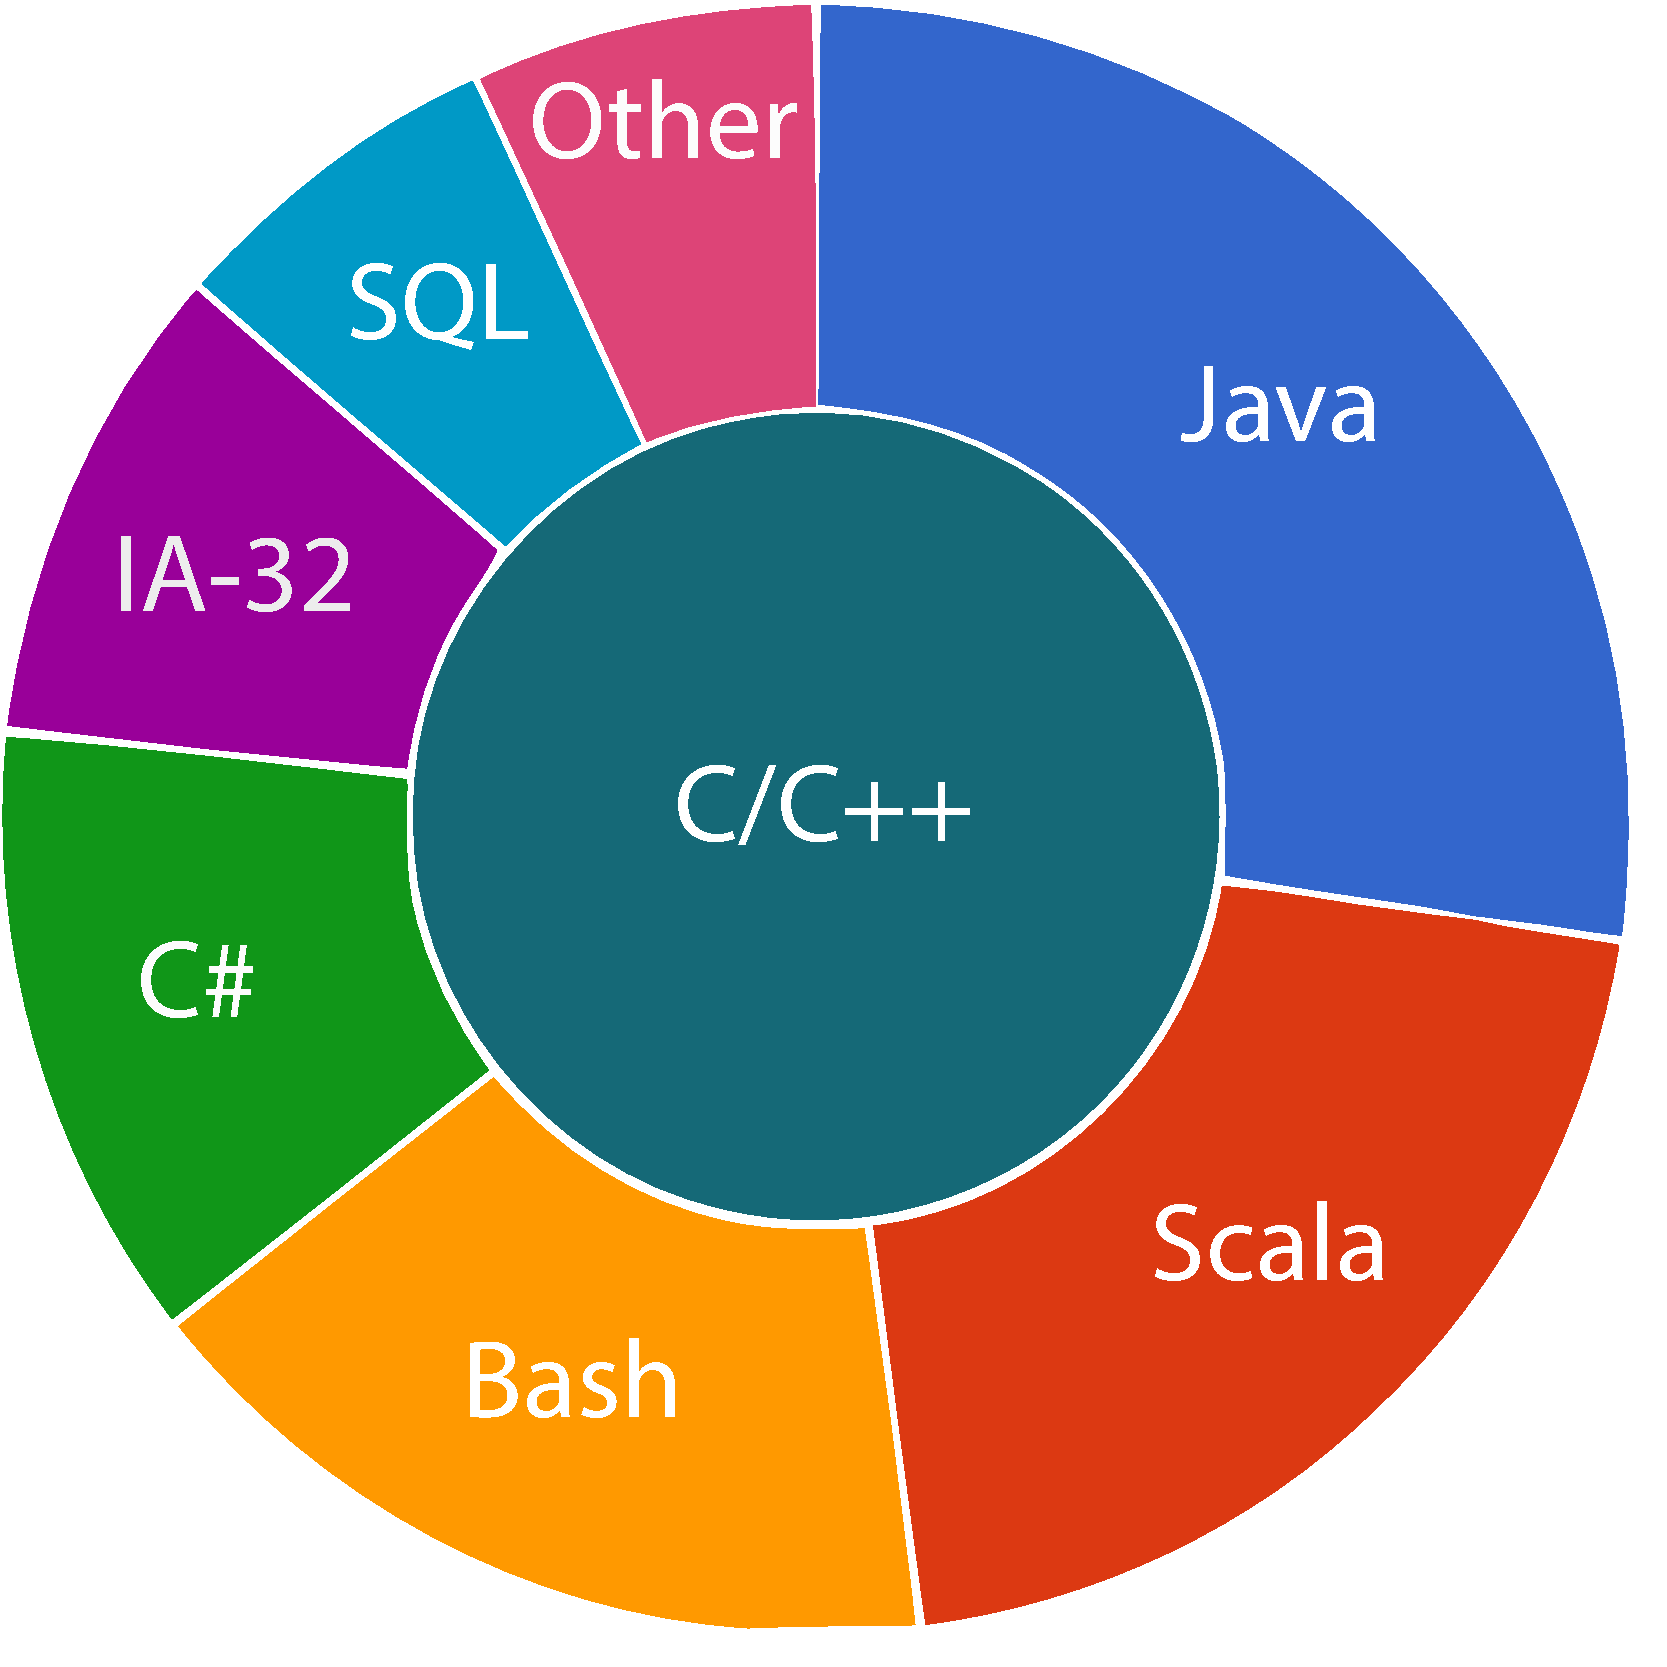
\includegraphics[width=0.18\paperwidth]{img/programming.pdf}
 %    \vspace{0.3cm}
    ~
    ~
     \section{Public Git}
    \href{https://github.com/Meraz}{github.com/Meraz}
    ~
    ~
  \section{OS Preference}
    \textbf{GNU/Linux}
\includegraphics[scale=0.40]{img/5stars.png}
    \textbf{Windows}
\includegraphics[scale=0.40]{img/4stars.png}
    \textbf{Unix}
\includegraphics[scale=0.40]{img/3stars.png}
    \textbf{MacOS}
\includegraphics[scale=0.40]{img/1stars.png}
    ~
    ~
 % \section{Personal Skills}
 %   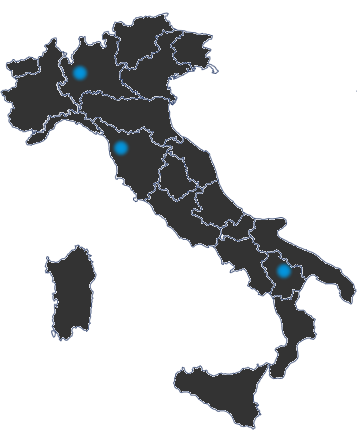
\includegraphics[scale=0.25]{img/italia.png}
 %   \includegraphics[scale=0.62]{img/personal.png}
 \section{Language}
    \textbf{Swedish}
\includegraphics[scale=0.40]{img/5stars.png}
    \textbf{English}
\includegraphics[scale=0.40]{img/4stars.png}
 ~
 ~
\end{aside}
\vspace{0.5cm}
\section{Personal Information}
\textbf{Date of birth} 1991-07-26

\textbf{Phone} +46 760 066 242

\textbf{Email} tilljander.rasmus@gmail.com

\textbf{Adress} Polhemsgatan 19A, 371 40, Blekinge, Sweden

\vspace{0.7cm}
\section{Experience}
\begin{entrylist}
  \entry
    {09/14 - 12/14}
    {Consultant, Software Engineer (4 months)}
    {HiQ, Karlskrona, Sweden}
    {Project based employment at HiQ Karlskrona AB in which I worked as a software developer at Ericsson AB in Karlskrona. The project included working with Ericssons internal systems, vaadin, scala and java.\\}
  \entry
    {11/11 - 09/01}
    {IT-Helpdesk (2 years, 1 month)}
    {Blekinge Institute of Technology, Sweden}
    {I answered questions and solved problems regarding the IT-services provided by Blekinge Institute of Technology. The work included working with services as the PayEx payment system and general problem solving with the printing system accessible by students.}
\end{entrylist}

\vspace{0.7cm}
\section{Education}
\begin{entrylist}
  \entry
    {2010 - 2016}
    {College}
    {Blekinge Institute of Technology, Karlskrona, Sweden}
    {Degee of Master of Science in Engineering: Game and Software Engineering\\
    Title of the Thesis:\emph{ Regional time stepping with two-scale PCISPH method}\\}
  \entry
    {2007 - 2010}
    {Highschool}
    {John Bauer Gymnasiet, Halmstad, Sweden}
    {Information Technology and Electrical Mathematics \\}
\end{entrylist}
}
\\
\begin{flushleft}
\emph{Mars 7th, 2015}
\end{flushleft}
\begin{flushright}
\emph{Rasmus Tilljander}
\end{flushright}

\end{document}
